\documentclass[11pt]{article}
\usepackage[margin=2.5cm]{geometry}
\usepackage{graphicx, hyperref}
\usepackage{amsthm, amsmath, amssymb}
\newtheorem{theorem}{Theorem}
\theoremstyle{definition}
\newtheorem{definition}{Definition}
\theoremstyle{remark}
\newtheorem{example}{Example}

\hypersetup{
	colorlinks=true,
	linkcolor=blue,
	citecolor=blue,
	urlcolor=blue
}

%For urls
\usepackage{url}

\title{Model Checking Real-Time Systems\\\small Written Abstract for the Seminar ``Recent Advances in Model Checking''}
\author{Vincent Trélat}
\date{}

\begin{document}
\maketitle	

\section*{Organizational information}
% - organization of the abstract and relation to the talk
% - motivation of why the others should care
% - formalities that you plan to use in your talk
% - an outlook of what to expect in your talk 
% - if possible, a paragraph on the relation to (some of) the other talks
This abstract is based on Chapter 29 of the Handbook of Model Checking~\cite{handbook}.
Section~\ref{sec:intro} first introduces and motivates model checking applied to real-time systems, building on~\cite[Chapter~29.1]{handbook}.
Section~\ref{sec:ta} gives some formal definitions from ~\cite[Chapter 29.2]{handbook} about timed-automata and related notions.

$\cdots$

\section{Introduction}\label{sec:intro}
$\cdots$

\section{Timed Automata}\label{sec:ta}
\paragraph{Preliminaries}\label{par:prelims}
In this chapter, time values are equated with non-negative real numbers of $\mathbb{R}_{\geq 0}$. A \emph{time sequence} is a finite or infinite non-decreasing sequence of time values. A \emph{timed word} over $\Sigma \times \mathbb{R}_{\geq 0}$ is a word over the alphabet $\Sigma$ sequentially paired with a time sequence. If the time sequence of a timed word is upper-bounded or converging, the timed word is said to be \emph{converging}.

Let $C$ be a finite set of variables called \emph{clocks}. A \emph{valuation} over $C$ is a mapping $v \colon C \to \mathbb{R}_{\geq 0}$. The set of valuations over $C$ is denoted $\mathbb{R}_{\geq 0}^C$ and $\text{\bf 0}_C$ denoted the valuation assigning 0 to every clock of C.

For any valuation $v$ and any time value $t$, the valuation $v + t$ denotes the valuation obtained by shifting all values of $v$ by $t$. For any subset $r$ of $C$, $v[r]$ is the valuation obtained by resetting all clocks of $r$ in $v$.

A \emph{constraint} $\varphi$ over $C$ is recursively defined by the following grammar:
\begin{equation*}
	\varphi ::= x \odot k\ |\ \varphi \land \varphi
\end{equation*}
where $x\in C$, $k \in \mathbb{Z}$ and $\odot \in \{<, \leq, =, \geq, >\}$.
The set of constraints over $C$ is denoted $\Phi(C)$.
We say that a valuation $v$ over $C$ satisfies $x \odot k$ when $v(x) \odot k$, and when $v$ satisfies a constraint $\varphi$, we write $v \models \varphi$. The set of valuations satisfying a constraint $\varphi$ is denoted $[\![\varphi]\!]_C$.

% There exists an extension to $x - y \odot k$ constraints called diagonal constraints, and the set of diagonal constraints is denoted $\Phi_d(C)$.

\paragraph{Timed Automata}\label{par:ta}
A timed automaton is basically a finite automaton with (real-time) constraints on the states.
The following formal definition is a reformulation of~\cite[Chapter 29.2, Definition 1]{handbook}.
\begin{definition}\label{def:ta}
	A \emph{Timed Automaton} (TA) $\mathcal{A}$ is the data $(L, l_0, C, \Sigma, I, E)$ where:
	\begin{itemize}
		\item $L$ is a finite set of \emph{locations} with initial location $l_0 \in L$;
		\item $C$ is a finite set of \emph{clocks};
		\item $\Sigma$ is a finite set of \emph{actions};
		\item $I \colon L \to \Phi(C)$ is an \emph{invariant mapping};
		\item $E \subseteq L \times \Phi(C) \times \Sigma \times 2^{C} \times L$ is a set of edges.
	\end{itemize}
	Any edge $(\ell, \varphi, a, r, \ell') \in E$ is denoted $\ell \xrightarrow{\varphi, a, r} \ell'$ where $\varphi$ is a \emph{guard}, and $r$ is a subset of clocks that are set to zero after taking the transition.
\end{definition}
An example of TA is given in Fig.~\ref{fig:ta_ex}.

\begin{figure}[ht]
\centering
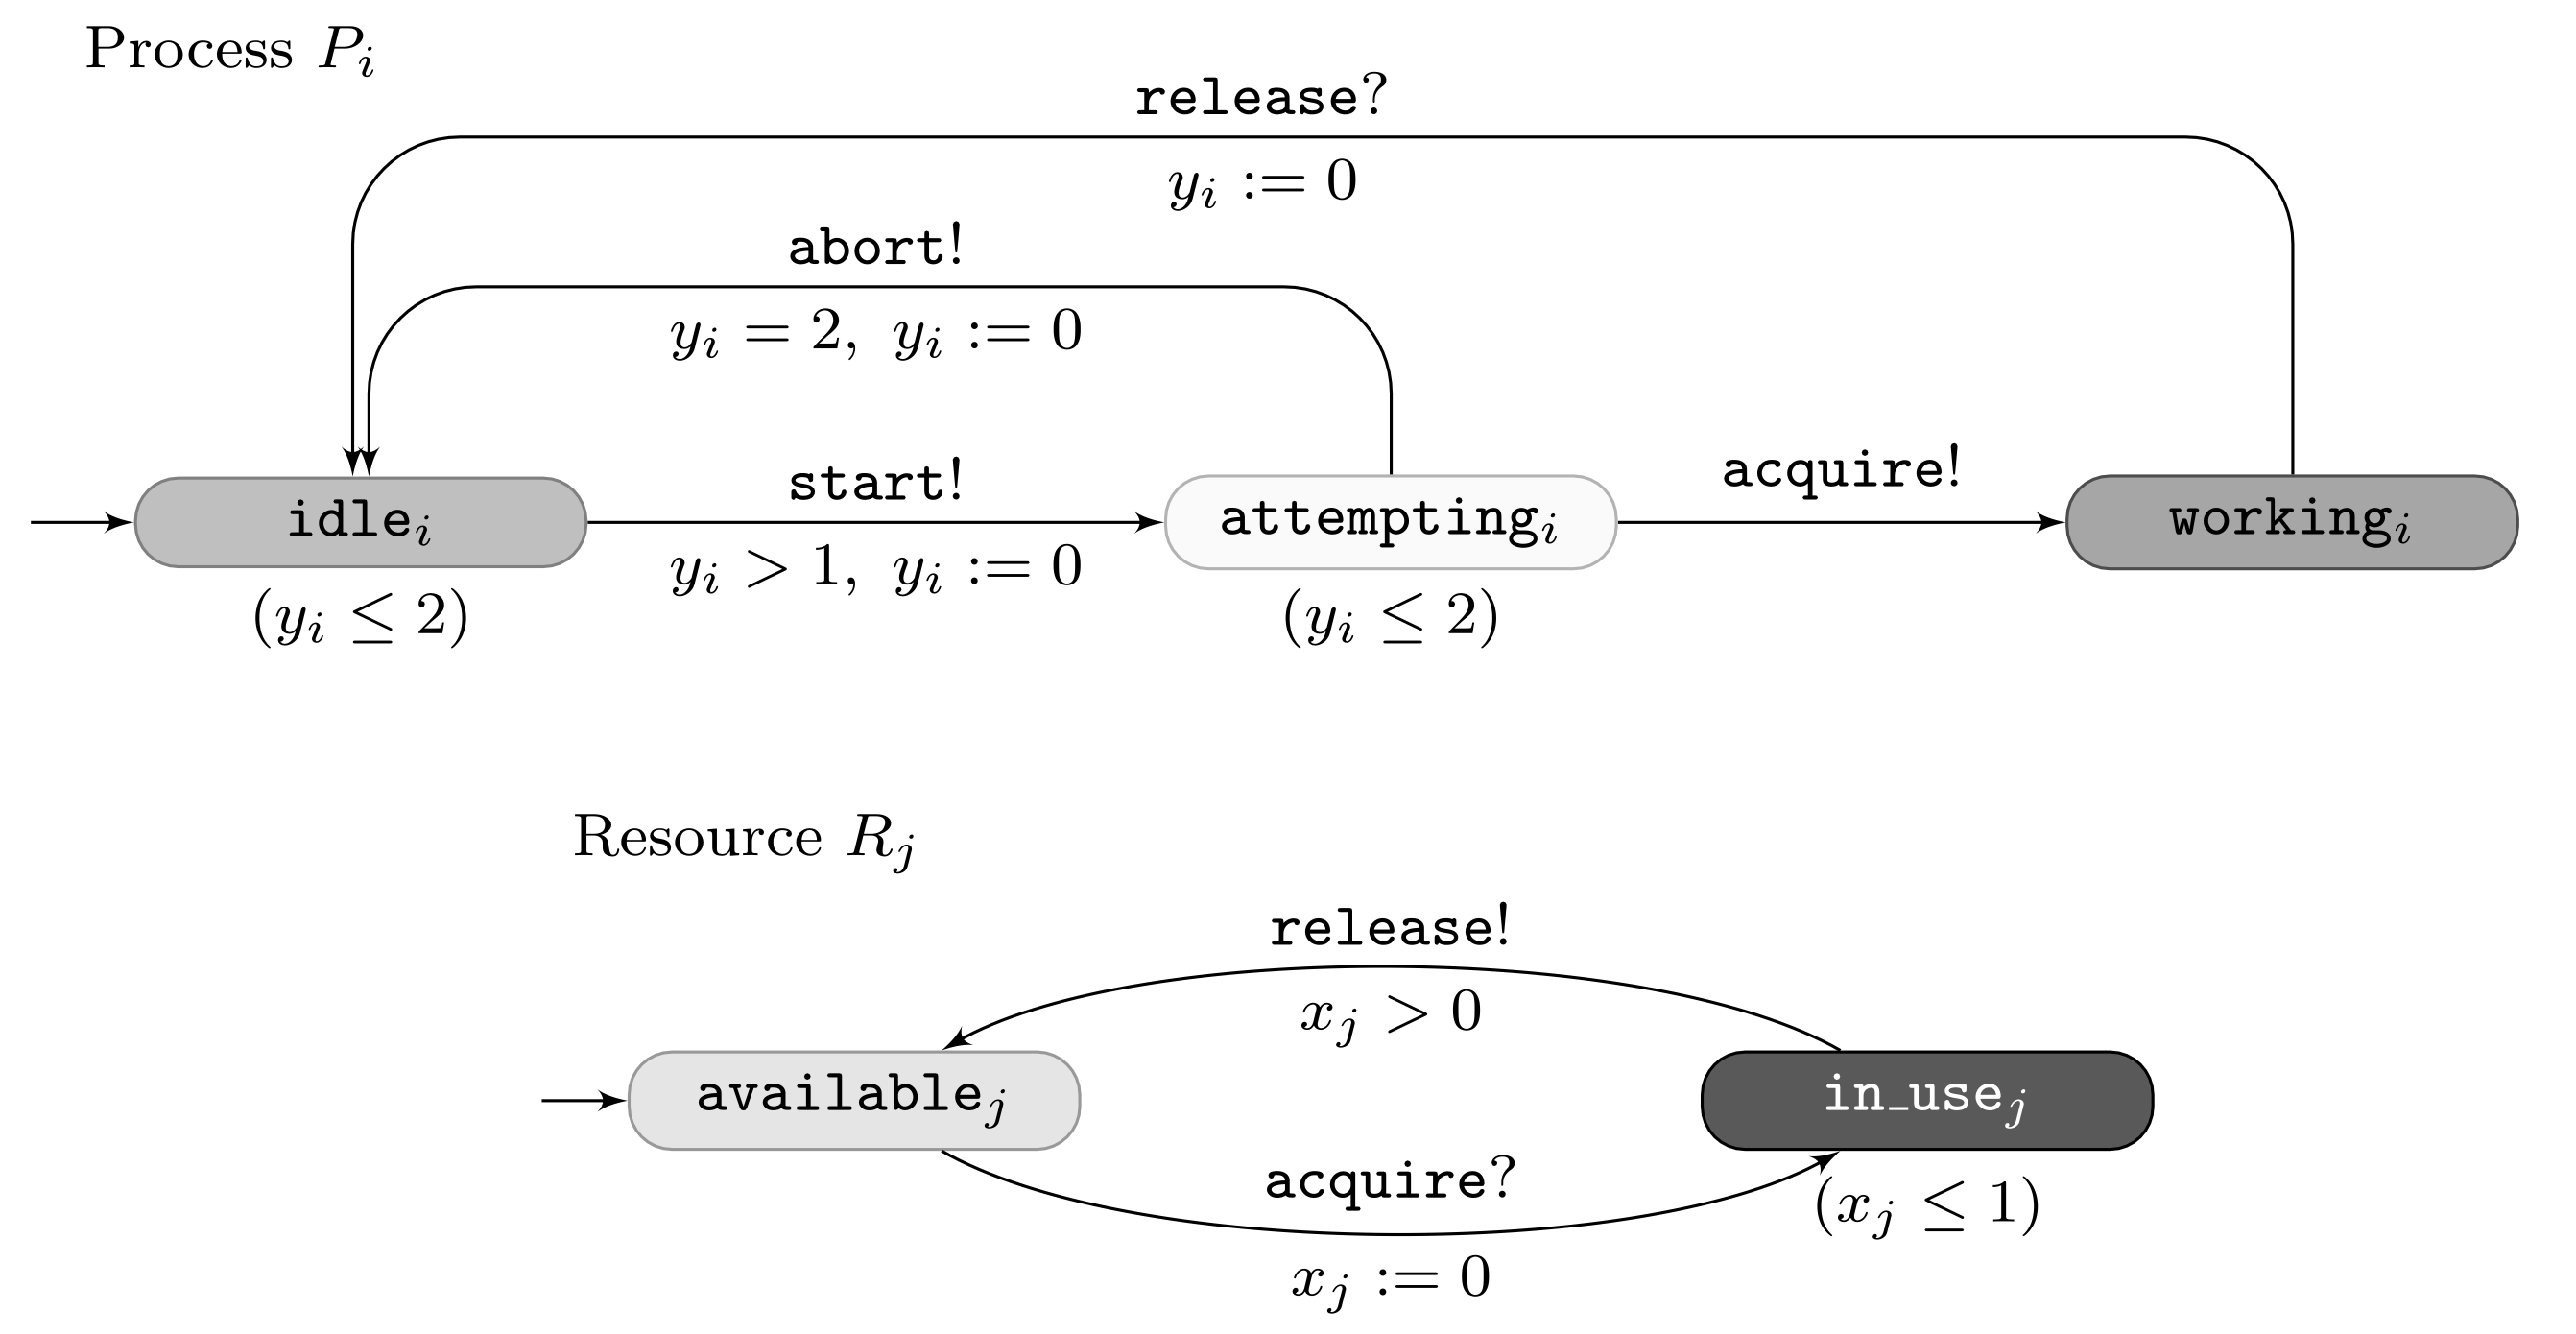
\includegraphics[width=.75\textwidth]{../img/TAex.png}
\caption{Two TA modeling processes which can use resources.}\label{fig:ta_ex}
\tiny{Figure taken from \cite[Chapter 29.2]{handbook}}
\end{figure}

\begin{definition}
	The \emph{operational semantics} of a TA $\mathcal{A} = (L, \ell_0, C, \Sigma, I, E)$ is the infinite-state timed transition system $[\![A]\!] = (S, s_0, \mathbb{R}_{\geq 0} \times \Sigma, T)$, where:
	\begin{itemize}
		\item $S := \{(\ell, v) \in L \times \mathbb{R}_{\geq 0}, v \models I(\ell)\}$ is the set of states | i.e.\ pairs of a location and a valuation such that the valuation is | satisfying the invariant and $s_0 := (\ell_0, \text{\bf 0}_C)$ is the inital state;
		\item $T := \{(\ell, v) \xrightarrow{d, a} (\ell', (v+d)[r]) \ | \ d \in \mathbb{R}_{\geq 0}, \forall d' \in [0, d], v + d' \models I(\ell) \land \exists \ell \xrightarrow{\varphi, a, r} \ell' \in E, v + d \models \varphi \}$ is the set of transitions that one can take by selecting a delay to be elapsed in $\ell$ and an edge of $\mathcal{A}$ to be taken after the delay\footnote{Provided that the invariant and the guard are satisfied!}.
	\end{itemize}
\end{definition}


\bibliographystyle{alpha}
\bibliography{ref}

\end{document}
